\documentclass[12pt,a4paper]{article}
\usepackage[utf8]{inputenc}
\usepackage[spanish]{babel}
\usepackage{amsmath}
\usepackage{amsfonts}
\usepackage{amssymb}
\usepackage{graphicx}
\usepackage{geometry}
\usepackage{booktabs}
\usepackage{float}
\geometry{left=2.5cm,right=2.5cm,top=2.5cm,bottom=2.5cm}

\begin{document}

\begin{titlepage}
    \centering
    \vspace*{1cm}
    
    
\includegraphics[scale=0.5]{Ulagos (1).png} 
    \vspace{2cm} 
    
    {\textbf{\Large Departamento de Ciencias de la Ingeniería}}
    
    \vspace{4.5cm}
    
    {\huge \textbf{Torque y Equilibrio}} \\[0.8cm]
    {\Large Laboratorio 2}
    
    \vfill
    
    \begin{flushright}
        \large
        \textbf{Asignatura:} Física Newtoniana \\[0.6cm]
        \textbf{Integrantes:} \\
        Matías Barrientos \\
        Kevin Bustos \\
        Emiliano Pino \\
        Tiare Osorio \\
        Luciano Gutierrez \\[0.6cm]
        \textbf{Fecha:} \today
    \end{flushright}
    
    \vspace*{1cm}
\end{titlepage}

\newpage
\pagenumbering{arabic}

% ==========================================
% CUERPO DEL INFORME
% ==========================================

\section{Marco Teórico}
El torque (representado por la letra griega tau, $\tau$) es la medida cuantitativa de la tendencia de una fuerza para causar o alterar la rotación de un cuerpo alrededor de un eje. Es una magnitud vectorial que se define como el producto cruz entre el vector de posición $\vec{r}$ (desde el eje de rotación hasta el punto de aplicación de la fuerza) y el vector fuerza $\vec{F}$. Matemáticamente se expresa como:
\begin{equation}
    \vec{\tau} = \vec{r} \times \vec{F}
\end{equation}
La magnitud del torque se calcula mediante la fórmula:
\begin{equation}
    \tau = r \cdot F \cdot \sin(\phi)
\end{equation}
donde $\phi$ es el ángulo entre el vector $\vec{r}$ y la fuerza $\vec{F}$.

En el contexto de este laboratorio, las fuerzas aplicadas (los pesos de las masas colgantes) son perpendiculares a la viga (es decir, $\phi = 90^\circ$ y $\sin(90^\circ)=1$), por lo que la magnitud del torque se simplifica a:
\begin{equation}
    \tau = r \cdot F
\end{equation}

\section{Procedimiento Experimental}
Para llevar a cabo la experiencia, se dispuso de una viga de madera con perforaciones (orificios A y B) y masas de diferentes magnitudes. Se utilizó una balanza de precisión para determinar la masa exacta de cada objeto y una cinta métrica para medir los brazos de palanca ($r$). A continuación, se detallan las masas utilizadas a lo largo de la experiencia y sus pesos respectivos. Para calcular el peso ($F$), se multiplicó la masa experimental por la aceleración de gravedad estándar ($g \approx 9.8 \, \text{m/s}^2$).

\begin{itemize}
    \item \textbf{Primera Parte (Eje en Orificio A):}
    \begin{itemize}
        \item Masa 1 ($m_1$): $0.100$ kg $\rightarrow$ Peso $\approx 0.98$ N
        \item Masa 2 ($m_2$): $0.203$ kg $\rightarrow$ Peso $\approx 1.99$ N
        \item Masa 3 ($m_3$): Varía de $0.303$ a $0.564$ kg $\rightarrow$ Peso $\approx 2.97$ a $5.53$ N
    \end{itemize}
    \vspace{0.2cm}
    \item \textbf{Segunda Parte (Eje en Orificio B):}
    \begin{itemize}
        \item Masa 1 ($m_1$): $0.048$ kg $\rightarrow$ Peso $\approx 0.47$ N
        \item Masa 2 ($m_2$): $0.101$ kg $\rightarrow$ Peso $\approx 0.99$ N
        \item Masa 3 ($m_3$): $0.820$ kg $\rightarrow$ Peso $\approx 8.04$ N
    \end{itemize}
\end{itemize}

Durante la primera parte, se suspendió la viga desde su orificio A y se buscaron las distancias necesarias para lograr el equilibrio rotacional ubicando las masas en distintas posiciones. En la segunda parte, se modificó el eje de rotación al orificio B, lo que introdujo el torque generado por la masa de la propia viga.

\vspace{0.5cm}
\begin{figure}[H]
    \centering
    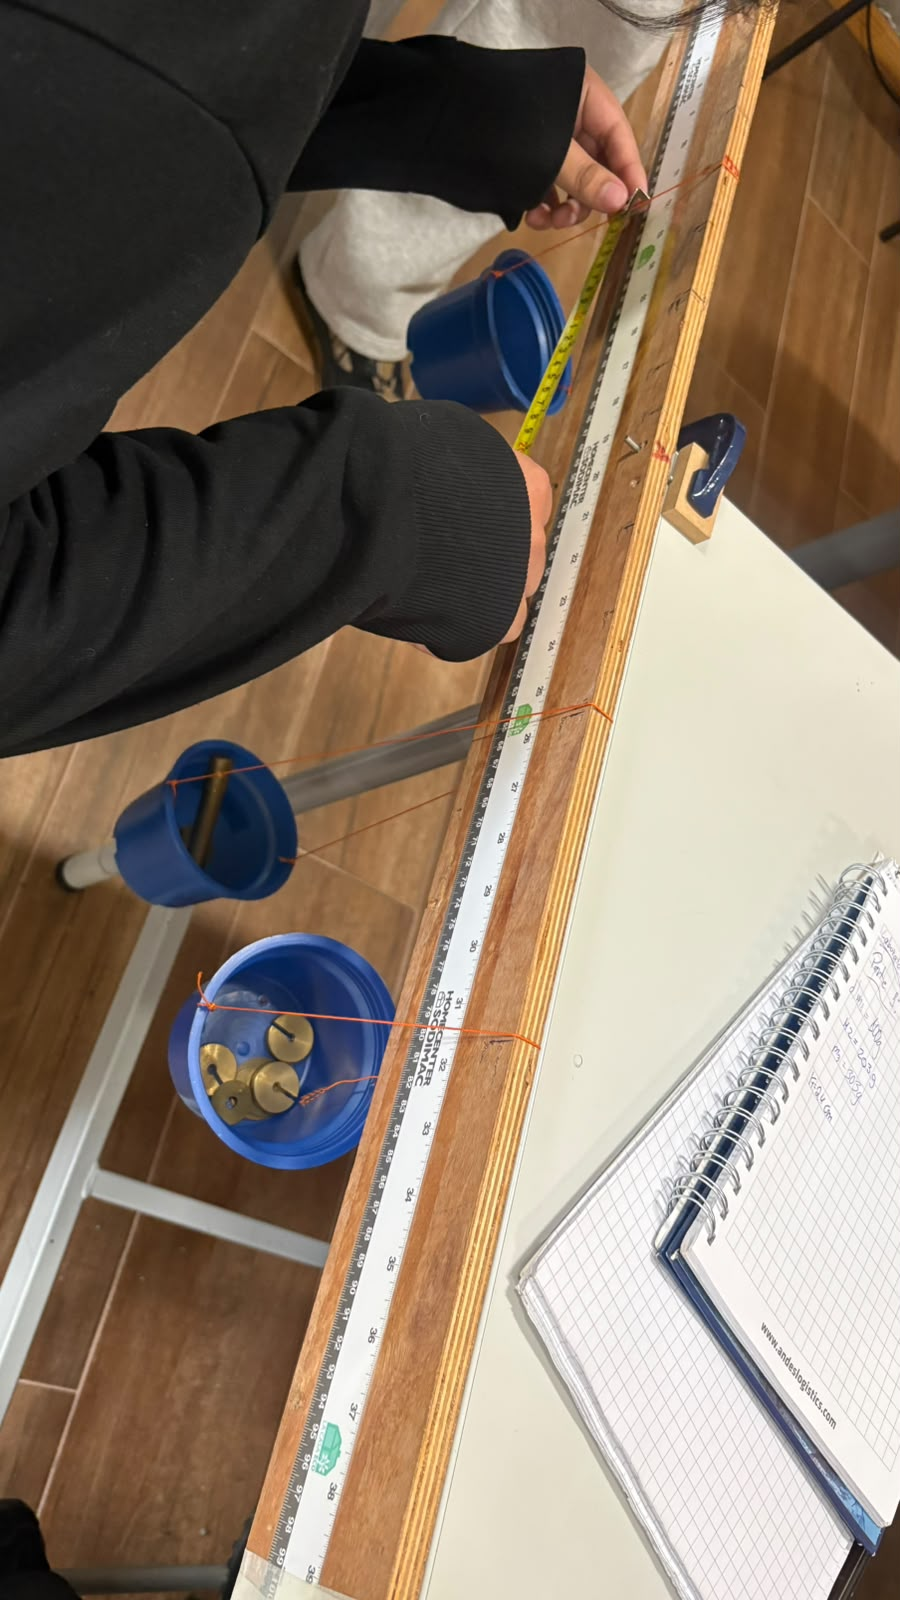
\includegraphics[angle=90, scale=0.25]{parte a.jpeg}
    \caption{Imagen del montaje experimental de la Primera Parte.}
\end{figure}

\begin{figure}[H]
    \centering
    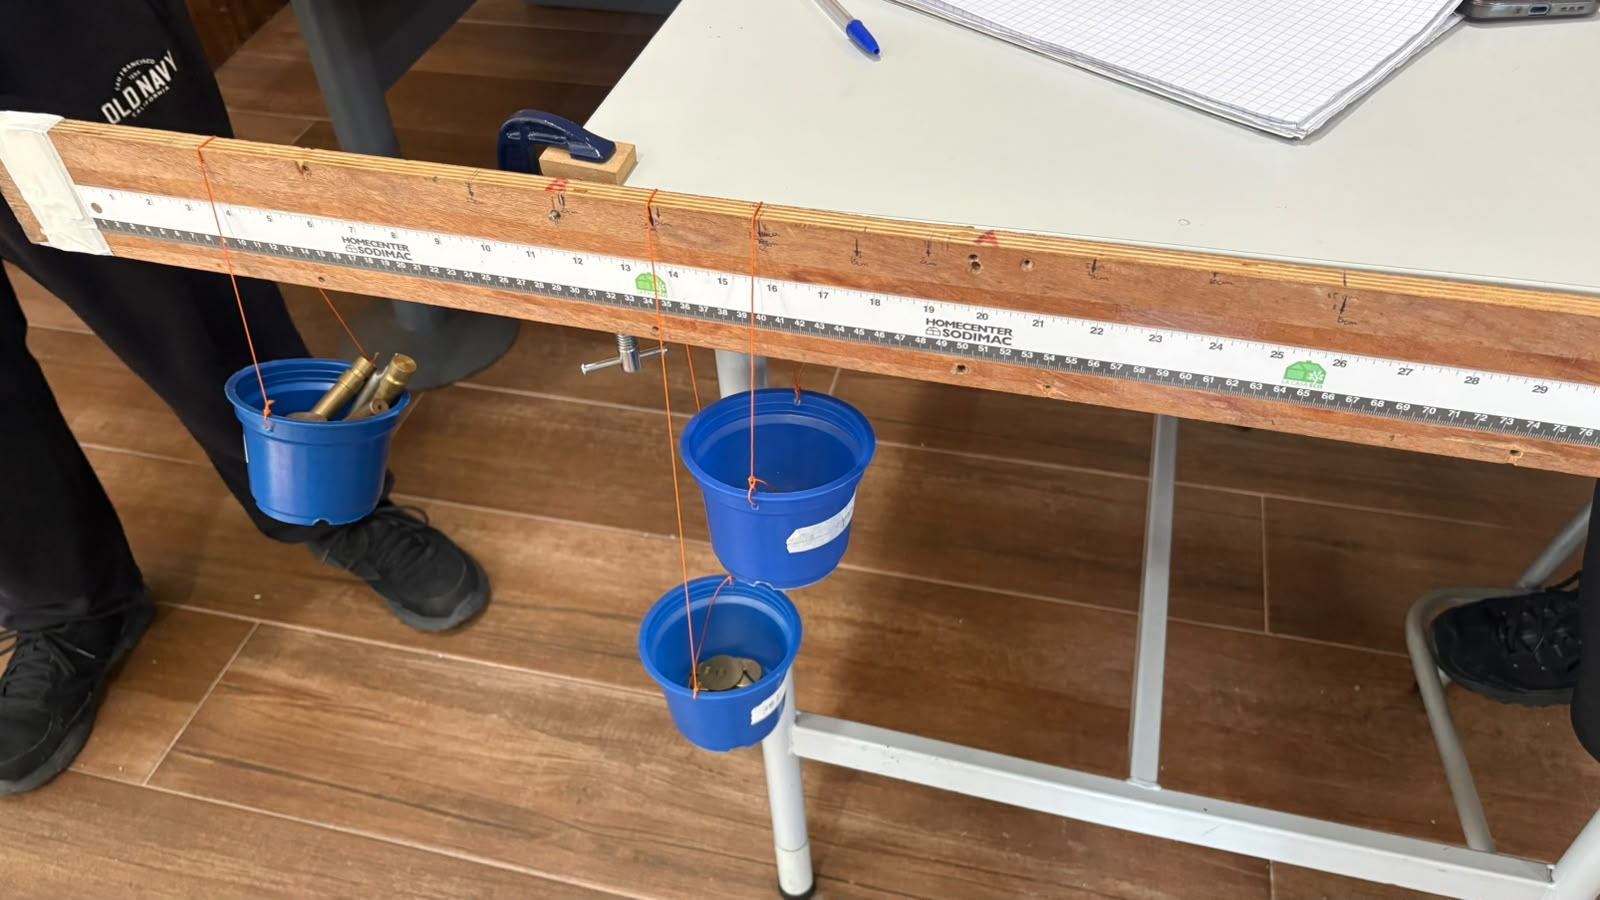
\includegraphics[scale=0.25]{parteb.jpeg}
    \caption{Imagen del montaje experimental de la Segunda Parte.}
\end{figure}

\newpage
\section{Resultados}
A continuación, se presentan los datos obtenidos en el laboratorio expresados en el Sistema Internacional (SI). Los valores presentados como ``Torque'' representan el producto directo de la masa por el brazo de palanca ($m \cdot r$).

\subsection{Primera Parte: Viga suspendida del orificio A}
Al suspender la viga desde su centro de gravedad (Orificio A), el torque ejercido por la propia viga es cero ($\tau_{\text{viga}} = 0$).

\begin{table}[H]
\centering
\begin{tabular}{lccc}
\toprule
\textbf{Parámetro} & \textbf{Caso d} & \textbf{Caso e} & \textbf{Caso f} \\
\midrule
$m_1$ (kg) & 0.100 & 0.100 & 0.100 \\
$r_1$ (m) & 0.150 & 0.300 & 0.300 \\
\textbf{Torque 1} ($kg \cdot m$) & 0.015 & 0.030 & 0.030 \\
\midrule
$m_2$ (kg) & 0.203 & 0.203 & 0.203 \\
$r_2$ (m) & 0.300 & 0.150 & 0.150 \\
\textbf{Torque 2} ($kg \cdot m$) & 0.0609 & 0.03045 & 0.03045 \\
\midrule
$m_3$ (kg) & 0.303 & 0.303 & 0.564 \\
$r_3$ (m) & 0.240 & 0.200 & 0.100 \\
\textbf{Torque 3} ($kg \cdot m$) & 0.07272 & 0.0606 & 0.0564 \\
\midrule
Torque viga ($kg \cdot m$) & 0 & 0 & 0 \\
\textbf{Sumatoria de torques} & \textbf{0.00318} & \textbf{-0.00015} & \textbf{0.00405} \\
\bottomrule
\end{tabular}
\caption{Datos experimentales correspondientes a la Primera Parte.}
\end{table}

\subsection{Segunda Parte: Viga suspendida del orificio B}
Al suspender la viga desde el orificio B, el centro de masa de la viga ejerce un torque adicional de $0.154 \, kg\cdot m$ que interactúa con las demás masas para mantener el sistema horizontal.

\begin{table}[H]
\centering
\begin{tabular}{lccc}
\toprule
\textbf{Parámetro} & \textbf{Caso g} & \textbf{Caso h} & \textbf{Caso i} \\
\midrule
$m_1$ (kg) & 0.048 & 0.048 & 0.048 \\
$r_1$ (m) & 0.050 & 0.100 & 0.200 \\
\textbf{Torque 1} ($kg \cdot m$) & 0.0024 & 0.0048 & 0.0096 \\
\midrule
$m_2$ (kg) & 0.101 & 0.101 & 0.101 \\
$r_2$ (m) & 0.150 & 0.050 & 0.050 \\
\textbf{Torque 2} ($kg \cdot m$) & 0.01515 & 0.00505 & 0.00505 \\
\midrule
$m_3$ (kg) & 0.820 & 0.820 & 0.820 \\
$r_3$ (m) & 0.200 & 0.200 & 0.200 \\
\textbf{Torque 3} ($kg \cdot m$) & 0.164 & 0.164 & 0.164 \\
\midrule
Torque viga ($kg \cdot m$) & 0.154 & 0.154 & 0.154 \\
\textbf{Sumatoria de torques} & \textbf{-0.00755} & \textbf{0.00015} & \textbf{-0.00465} \\
\bottomrule
\end{tabular}
\caption{Datos experimentales correspondientes a la Segunda Parte.}
\end{table}

\section{Análisis de Datos}
A partir de los resultados obtenidos, se observa que la sumatoria de torques en ambas partes del experimento es muy cercana a cero ($\sum (m \cdot r) \approx 0$). Para que estos datos estén expresados rigurosamente en unidades de Newton-metro (N$\cdot$m), los valores calculados deben ser multiplicados por la aceleración de gravedad ($g \approx 9.8 \, \text{m/s}^2$). Dado que la gravedad actúa como una constante sobre todo el sistema, la proporcionalidad se mantiene y demuestra el equilibrio rotacional ($\sum \tau \approx 0$).

Las pequeñas variaciones que impiden que la sumatoria sea exactamente cero se pueden atribuir a diversas fuentes de error presentes en el desarrollo experimental. Entre los errores sistemáticos se identifica un posible defecto de calibración en la cinta métrica o la existencia de rozamiento en el eje de rotación que no fue considerado en el modelo teórico. Por otro lado, los errores aleatorios se asocian principalmente a dificultades visuales (errores de paralaje) al intentar determinar la horizontalidad exacta de la viga y al ubicar las masas en las marcas precisas de la regla métrica.

\section{Conclusiones}
Tras la realización del laboratorio, se comprobó experimentalmente la condición de equilibrio rotacional para un cuerpo rígido. Se evidenció que la suma de los torques debido a todas las fuerzas externas que actúan sobre la viga es cero, validando así el modelo teórico impartido en clases. 

Las implicancias físicas de estos resultados demuestran que el punto de aplicación de una fuerza es tan importante como su magnitud al momento de generar rotación, lo cual se observó claramente al cambiar el eje de rotación del orificio A al orificio B, donde la propia masa de la viga comenzó a ejercer un torque significativo. 

A pesar de existir una leve dispersión en la sumatoria final de los torques, el modelo teórico resulta ser altamente válido para el rango de datos medidos. Para mejorar la precisión en futuras sesiones, se sugiere incorporar un nivel de burbuja para garantizar la horizontalidad perfecta de la viga, así como minimizar la fricción en el eje de rotación utilizando lubricantes o rodamientos de mayor precisión.

\section{Referencias}
\begin{itemize}
    \item Young, H. D., \& Freedman, R. A. (2018). \textit{Física Universitaria con Física Moderna} (14.ª ed., Vol. 1). Pearson Educación.
    \item Guía de Laboratorio N$^\circ$2: Torque y equilibrio. Departamento de Física, Universidad de Los Lagos.
\end{itemize}

\end{document}
